\chapter{Interactive Program Synthesis}
\label{ch:interactive}

The key challenge of PBE and, more generally, programming with under-specifications, is \emph{intent ambiguity}.
Examples are an inherently ambiguous form of specification.
A typical industrial DSL usually may contain up to $10^{20}$ programs that are consistent with a given input-output
example~\cite{singh2012synthesizing}.
The underlying PBE system might end up synthesizing an unintended program that is consistent with the examples provided
by the user but does not generate the intended results on some other inputs that the user cares about.
In \citeyear{pbd-fail}, \citeauthor{pbd-fail} presented a critical discussion of PBE systems noting that adoption
of PBE systems is not yet widespread, and proposing that this is mainly due to lack of usability
and confidence in such systems~\cite{pbd-fail}.
We have observed the issues of confidence, transparency, and debuggability to arise in most interactions with PBE-based
synthesis systems.

In the past, intent ambiguity in PBE has been primarily handled by imposing a sophisticated ranking on the
DSL~\cite{cav:ranking}.
While ranking goes a long way in avoiding undesirable interpretations of the user's intent, it is not a complete
solution.
For example, FlashFill is designed to cater to users that care not about the program but about its behavior on the small
number of input rows in the spreadsheet.
Such users can simply eye-ball the outputs of the synthesized program and provide another example if they are incorrect.
However, this becomes much more cumbersome (or impossible) with a larger spreadsheet.%
\footnote{John Walkenbach, famous for his Excel textbooks, labeled \ff as a ``controversial'' feature.
    He wrote: \textit{``It's a great concept, but it can also lead to lots of bad data. I think many users will look at
        a few ``flash filled'' cells, and just assume that it worked. But my preliminary tests leads me to this
        conclusion: Be very careful.''}~\cite{walkenbach:controversial}}
Moreover, inspecting the synthesized program directly also does not establish enough confidence in it even if the user
knows programming.
Two main reasons for this are (i) program readability,%
\footnote{Stephen Owen, a certified MVP (``Most Valued Professional'')
  in Microsoft technologies, said the following of a program
  synthesized by \fe: \textit{``If you can understand this, you’re a better person than I am.''}~\cite{mvp:complaint}}
and (ii) the users' uncertainty in the desired intent due to hypothetical unseen corner cases in the data.

Due to ambiguity of intent in PBE, the standard user interaction model in this setting is for the user to provide
constraints \emph{iteratively} until the user is satisfied with the synthesized program or its behavior on the known
inputs.
However, most work in this area, including FlashFill and FlashExtract, has not been formally modeled as an iterative
process.
In this work, I describe our interactive formulation of program synthesis that leverages the inherent iterative nature
of synthesis from under-specifications, as well as multiple novel techniques for intent disambiguation and user
interaction models that leverage the innate strengths of this interactive formulation.

In \Cref{sec:interactive:problem}, I formally introduce the problem of \emph{interactive program synthesis}, wherein an
application-specific \emph{synthesis session state} is kept after each iteration.
This state is used to improve the transparency, performance, and debuggability of the synthesis process via various
means, including proactive feedback to the user, directing the user toward better examples, and speeding up the next
synthesis iterations incrementally.

In \Cref{sec:interactive:models}, I describe our exploration and evaluation of user interaction models that aim to
improve the transparency of the iterative synthesis process.
Our proposed two novel interaction models alleviate above\hyp{}mentioned transparency concerns
by exposing more information to the user in a form that can be easily understood and acted upon.
These models help resolve ambiguity in the example\hyp{}based specification, thereby increasing
user's trust in the results produced by the PBE engine.
The first model, \emph{Program Navigation}, allows the user to navigate
between all programs synthesized by the underlying PBE engine (as opposed to displaying only the
top-ranked program) and to pick one that is intended.
We leverage the implicit sharing present in a VSA~(\Cref{ch:vsa}) to create a navigational interface that allows the
user to select from different ranked choices for various parts of the top-ranked program.
Furthermore, these programs are paraphrased in English for easy readability.
The second model, \emph{Conversational Clarification}, is based on active learning.
In it, the system asks questions to the user to resolve ambiguities in the user's
specification with respect to the available test data.
These questions are generated after the PBE engine has synthesized multiple programs that are consistent with the
user-provided examples.
The system executes these multiple programs on the test data to identify any discrepancies in the execution and uses
that as the basis for asking questions to the user.
The user responses are used to refine the initial example-based specification and the
process of program synthesis is repeated.

\Cref{sec:interactive:feedback} builds on the ideas of Conversational Clarification, generalizing it into a universal
formal technique that is applicable to an arbitrary interactive synthesis process -- \emph{feedback-based synthesis}.
It builds on our interactive problem definition from \Cref{sec:interactive:problem}.
I present a method for leading the user toward the examples with maximum disambiguation potential, and discuss our
usage of feedback-based synthesis in PROSE-based applications.

Finally, in \Cref{sec:interactive:incremental}, I show how the same problem formulation can be used to improve the
performance of the synthesis process.
The standard PBE model requires the user to refine her intent in iterative rounds by providing additional constraints on
the current candidate program.
The standard approach has been to re-run the synthesizer afresh with the conjunction of the original constraints and the
new constraints.
In this work, I introduce an alternative technique: leveraging the \emph{interpretation of previously learned VSA as a
sub-language~(\Cref{sec:vsa:language})} to carry out the new round of synthesis on a smaller program space.

\section{Problem Definition}
\label{sec:interactive:problem}

In this section, I extend the conventional program synthesis problem definition~(\Cref{problem:syn:general}) to
incorporate learner-user interaction.
It allows us to model the inherent interactive workflow in a first-class manner in the program synthesis formalism and
associated techniques.

\begin{problem}[Interactive Program Synthesis]
    Let $\dsl$ be a DSL, and $N$ be a symbol in $\dsl$.
    Let $\synalgorithm$ be an \emph{inductive synthesis algorithm} for $\dsl$, which solves problems of type
    $\mathsf{Learn}\left(N, \spec\right)$ where $\spec$ is an \emph{inductive spec} on a program rooted at $N$.
    The specs $\spec$ are chosen from a fixed class of \emph{supported spec types} $\Phi$.
    The result of $\mathsf{Learn}\left(N, \spec\right)$ is some set $\vsa$ of programs rooted at $N$ that are consistent
    with $\spec$.

    Let $\spec^{*}$ be a spec on the output symbol of $\dsl$, called a \emph{task spec}.
    A~\textbf{$\bm{\spec^{*}}$-driven interactive program synthesis process} is a finite series of 4-tuples
    $\langle N_0, \spec_0, \vsa_0, \Sigma_0\rangle, \dots, \langle N_m, \spec_m, \vsa_m, \Sigma_m\rangle$, where
    \begin{itemize}[nosep]
        \item Each $N_i$ is a nonterminal in $\dsl$,
        \item Each $\spec_i$ is a spec on $N_i$,
        \item Each $\vsa_i$ is some set of programs rooted at $N_i$ s.t. $\vsa_i \models \spec_i$,
        \item Each $\Sigma_i$ is an \textbf{interaction state}, explained below,
    \end{itemize}
    which satisfies the following axioms for any program $P \in \dsl$:
    \begin{enumerate}[nosep, label=\textbf{\Alph*.}]
        \item $(P \models \spec^{*}) \Rightarrow (P \models \spec_i)$ for any $0 \le i \le m$;
        \item $(P \models \spec_j) \Rightarrow (P \models \spec_i)$ for any $0 \le i < j \le m$ s.t. $N_i = N_j$.
    \end{enumerate}
    We say that the process is \textbf{converging} iff the top-ranked program of the last program set in the process
    satisfies the task spec:
    \[
        P^{*} = \mathsf{Top}_h\left(\vsa_m, 1\right) \models \spec^{*}
    \]
    and the process is \textbf{failing} iff the last program set is empty: $\vsa_m = \emptyset$.

    An \textbf{interactive synthesis algorithm} $\widehat{\synalgorithm}$ is a procedure (parameterized by $\dsl$, $\synalgorithm$, and $h$)
    that solves the following problem:
    \[
        \mathsf{LearnIter}\colon \left\{
        \begin{aligned}
            \langle N_0, \spec_0, \bot\rangle &\mapsto \langle \vsa_0, \Sigma_0\rangle \\
            \langle N_i, \spec_i, \Sigma_{i-1} \rangle &\mapsto \langle \vsa_i, \Sigma_i\rangle, \quad i > 0
        \end{aligned}
        \right.
    \]
    In other words, at each iteration $i$ the algorithm receives the $i^{\text{th}}$ learning task $\langle N_i, \spec_i\rangle$ and its own
    interaction state $\Sigma_{i-1}$ from the previous iteration.
    The type and content of $\Sigma_i$ is unspecified and can be implemented by $\widehat{\synalgorithm}$ arbitrarily.
    \label{problem:interactive}
\end{problem}

\begin{defn}
    An interactive synthesis algorithm $\widehat{\synalgorithm}$ is \emph{complete} iff for any task spec $\spec^{*}$:
    \begin{itemize}[nosep]
        \item If $\exists P \in \dsl$ such that $P \models \spec^{*}$ then $\widehat{\synalgorithm}$ eventually
            converges for any $\spec^{*}$-driven interactive synthesis process.
        \item Otherwise, $\widehat{\synalgorithm}$ eventually fails for any $\spec^{*}$-driven interactive synthesis
            process.
    \end{itemize}
\end{defn}

The notion of an interactive synthesis process formally models a typical learner-user interaction where $\spec^{*}$
describes the desired program.
The task spec is not know to the synthesizer -- it is an ``ideal spec'' that would unambiguously specify the user
intent.
The general nature of definitions in \Cref{problem:interactive} allows many different implementations for
$\widehat{\synalgorithm}$.
In addition to completeness, different implementations (and choices for the state $\Sigma$) strive to satisfy different
\emph{performance objectives}, such as:
\begin{itemize}[nosep]
    \item Number of interaction rounds (e.g. examples) $m$,
    \item The total amount of information communicated by the user,
    \item Cumulative execution time of all $m+1$ learning calls.
\end{itemize}
In the rest of this chapter, I present several specific instantiations of interactive synthesis algorithms that
optimize these objectives.

\section{User Interaction Models}
\label{sec:interactive:models}

This section formally introduces \emph{Program Navigation} and \emph{Conversational Clarification} -- our proposed user
interaction models to improve the transparency of intent disambiguation process.
We have built a prototype UI called PROSE \FlashProg,\footnote{Available at
\url{https://prose-playground.cloudapp.net}.} which incorporates both interaction models, and used it to conduct a user
study.
In the study, we asked participants to extract structured data from semi-structured text files using \FlashProg.
We observe that participants perform more correct extraction when they
make use of the new interaction models.

To our surprise, participants preferred \ConversationalClarification over \ProgramNavigation slightly more even though
past case studies suggested that users wanted to look at the synthesized programs.
We believe this is explained by the fact that
because \ConversationalClarification is a \emph{proactive} interface that asks clarifying questions, whereas
\ProgramNavigation is a \emph{reactive} interface that expects an explicit correction of a mistake.

\subsection{User Interface}

\Cref{fig:interactive:ui:overview} shows a \FlashProg window after providing several examples (on the left), and after
invoking the learning process (on the right).
The \FlashProg window consists of 3 sections: \TopToolbarView (1), \InputTextView (2), and \PBEView (3).

\begin{figure}[p!]
    \centering
    \uwsinglespace
    \begin{tcbraster}[beamer, raster columns=1, size=minimal]
        \centering
        \tcbincludegraphics[scale=0.8]{figures/FlashProgMod4-before}
    \end{tcbraster}
    \vspace*{\baselineskip}
    \begin{tcbraster}[beamer, raster columns=1, size=minimal]
        \centering
        \tcbincludegraphics[scale=0.8]{figures/FlashProgMod4}
    \end{tcbraster}
    \caption{\FlashProg UI with PBE Interaction View in the ``Output'' mode, before and after the learning process.
        1 -- \TopToolbarView, 2 -- \InputTextView, 3 -- \PBEView.}
    \label{fig:interactive:ui:overview}
\end{figure}

% The \TopToolbarView contains: (a) an input button to open and upload files,
% (b) a button that resets \FlashProg to an initial state,
% (c) undo/redo buttons as expected,
% and (d) a ``Results'' button to download the output as a CSV file for further processing.

The \InputTextView is the main area.
It gives users the ability to provide examples by highlighting desired sections of the document, producing a set of
nested colored blocks.
Additionally, users may omit the structure boundary and only provide examples for the fields as shown in
\Cref{fig:interactive:ui:overview}.
After an automated learning phase, the output of the highest ranked program is displayed in the Output pane.
Each new row in the output is also matched to the corresponding region of the original document that is highlighted with
dimmer colors.
The user can also provide \emph{negative examples} by clicking on previously marked regions to communicate to the PBE
system that the region
should not be selected as part of the output.

The \PBEView is a tabbed pane giving users an opportunity to interact with the PBE system in three different ways: (i)
exploring the produced output,
(ii) exploring the learned program set paraphrased into English in the program viewer (\ProgramNavigation),
and (iii)~engaging in an active learning session through the ``Disambiguation'' feature
(\ConversationalClarification).\footnote{
    Note that throughout this chapter, I refer to the ``disambiguation'' as an overall problem of selecting the program
    that realizes user's intent in PBE.
    However, in our UI we use the word ``Disambiguation'' as a header of a pane with one iteration of the
    \ConversationalClarification process.
    We found that it describes \ConversationalClarification most lucidly to the users.
    % Hereinafter in the chapter, I refer to the ``Disambiguation pane'' in our UI
    % if the context does not facilitate any confusion with the ``disambiguation problem''.
}

The Output pane displays the current state of data extraction result either as a relational table or as a tree.
To facilitate exploration of the data, the \InputTextView is scrolled to
the source position of each cell when the user hovers over it.
The user can also mark incorrect table rows as negative examples.

\begin{figure}[t]
    \centering
    \uwsinglespace
    \begin{tcbraster}[beamer, raster columns=1, size=minimal]
        \centering
        \tcbincludegraphics[scale=0.6]{figures/paraphrasing}
    \end{tcbraster}
    \caption{\ProgramNavigationTab of the PROSE \FlashProg.
        It shows the extraction programs that were learned in the session in \Cref{fig:interactive:ui:overview}.
        They are paraphrased in English and indented.}
    \label{fig:interactive:ui:paraphrasing}
\end{figure}

\begin{figure}[t]
    \uwsinglespace
    \begin{tcbraster}[beamer, raster columns=1, size=minimal]
        \centering
        \tcbincludegraphics[scale=0.7]{figures/05-author-list-alternative-program}
    \end{tcbraster}
    \caption{\ProgramNavigationTab \& alternative subexpressions.}
    \label{fig:interactive:ui:alternatives}
\end{figure}

\begin{figure}[t]
    \begin{tcbraster}[beamer, raster columns=1, size=minimal]
        \centering
        \tcbincludegraphics[scale=0.7]{figures/07-author-disambiguation-full}
    \end{tcbraster}
    \caption{\ConversationalClarification being used to disambiguate different programs that extract individual
    authors.}
    \label{fig:interactive:ui:disambiguation}
\end{figure}

The Program viewer pane (\Cref{fig:interactive:ui:paraphrasing}) lets users explore the learned programs.
We concisely describe regexes that are used to match strings in the input text.
For instance, ``\texttt{Words/dots/hyphens $\concat$ WhiteSpace}''
represents \texttt{[-.\textbackslash p{Lu}\textbackslash  p{Ll}]+o\textbackslash p{Zs}+} (viewable in code mode).
To facilitate understanding of these regexes, when the user hovers over
part of a regex, our UI highlights matches of that part in the text.
In \Cref{fig:interactive:ui:paraphrasing}, \texttt{Name-Struct} refers to the region
between two consecutive names; \texttt{City-Struct} refers to the region
between \texttt{City} and the end of the enclosing \texttt{Name-Struct} region.
Learned programs reference these regions to extract data.
For instance, \texttt{Phone} is learnt relatively to enclosing
\texttt{City-struct} region: ``\texttt{second line}'' refers to the line in the \texttt{City} region.
In addition, clicking on the triangular marker opens a list of alternative suggestions for each subexpression.
We show number of highlights that will be added (or changed/removed) by the alternative
program as a +number (or a -number).
If the program is incorrect, the user can replace some expressions with alternatives from the suggested list
(\Cref{fig:interactive:ui:alternatives}).

The Disambiguation pane (\Cref{fig:interactive:ui:disambiguation}) presents the \ConversationalClarification interaction
model.
The PBE engine often learns multiple programs that are consistent with the examples but produce different outputs
on the rest of the document.
In such cases, this difference is highlighted and user is presented with an option to choose between the two behaviors.
Choosing one of the options is always equivalent to providing one more example (either positive or negative), thereby
invoking the learning again on the extended specification.

\subsection{\ProgramNavigation}
The two key challenges in \ProgramNavigation are: paraphrasing of the DSL programs in English, and providing alternative
suggestions for program expressions.

\paragraph{Templating language}
To enable paraphrasing, we implemented a high\hyp{}level templating language, which maps \emph{partial programs} into
\emph{partial English phrases}.
\citeauthor{pbd-fail} stated~\cite{pbd-fail}:
\begin{quote}
    \textit{``Users complained about arcane
        instructions such as ``set the \texttt{CharWeight} to $1$'' (make the text bold).
        $[\ldots]$ SMARTedit users also thought a higher-level description such as ``delete all
    hyperlinks'' would be more understandable than a series of lower level editing commands.''}
\end{quote}
Our template-based strategy for paraphrasing avoids arcane instructions by using \emph{context-sensitive formatting
rules}, and avoids low-level instructions by using \emph{idioms}, solving the aforementioned two
problems~\cite{flashprog}.

\paragraph{Program alternatives}
To enable alternatives, we record the original candidate program set for each subexpression in the chosen program.
Since it is represented as a VSA, we can easily retrieve a subspace of alternatives for each program subexpression, and
apply the domain-specific ranking function on them.
The top $5$ alternatives are presented to the user.

\subsection{\ConversationalClarification}
\ConversationalClarification selects examples based on different outputs produced by generated programs.
Each synthesis step produces a VSA of ambiguous programs that are consistent with the given examples.
\ConversationalClarification iteratively replaces the subexpressions of the top-ranked program with its top $k$
alternatives from the VSA.
The clarifying question for the user is based on the \emph{first discrepancy} between the outputs of the currently
selected program $P$ and an alternative program $P'$.
Such a discrepancy can have three possible manifestations:
\begin{itemize}
    \item The outputs of $P$ and $P'$ match until $P$ selects a region $r$, which does not intersect any selection of
        $P'$.
        This leads to the question ``Should $r$ be highlighted or not?''
    \item The outputs of $P$ and $P'$ match until $P'$ selects a region $r'$, which does not intersect any selection of
        $P$.
        This leads to the question ``Should $r'$ have been highlighted?''
    \item The outputs of $P$ and $P'$ match until $P$ selects a region $r$, $P'$ selects a different region $r'$, and
        $r$ intersects
        $r'$.
        This leads to the question ``Should $r$ or $r'$ be highlighted?''
\end{itemize}
For better usability (and faster convergence), we merge the three question types into
one, and ask the user ``What should be highlighted: $r_1$, $r_2$, or nothing?''
Selecting $r_1$ or $r_2$ would mark the selected region as a positive example.
Selecting ``nothing'' would mark both $r_1$ and $r_2$ as negative examples.
After selecting an option, we convert the choice into one or more examples, and invoke a new synthesis process.

\subsection{Evaluation}
\newcommand{\plural}[3]{\ifnum 1=#1 #1 #2\xspace\else #1 #3\xspace\fi}
\newcommand{\ifequal}[4]{\ifnum #1=#2 #3\else #4\fi}

\newcommand{\numPeopleSurvey}{29}
\newcommand{\numPeopleOptin}{80}
\newcommand{\numPeopleEarlyTesters}{4}
\newcommand{\numWomen}{4}
\newcommand{\numMen}{25}
\newcommand{\minAge}{19}
\newcommand{\maxAge}{34}
\newcommand{\minProgrammingExperienceYears}{0}
\newcommand{\maxProgrammingExperienceYears}{less than 20 years}
\newcommand{\minDataExtractionFrequency}{never or several times a year}
\newcommand{\maxDataExtractionFrequency}{every day}
\newcommand{\percentagePreferenceFlashProg}{72}
\newcommand{\recommendFlashProgPercentage}{100}
\newcommand{\excitementPercentToHaveFlashProgFourOrFive}{79}
\newcommand{\percentageUsingProgramViewer}{45}
\newcommand{\percentageUsingDisambiguation}{93}
\newcommand{\usefulnessProgramViewer}{4.2}
\newcommand{\usefulnessProgramViewerStdDev}{2.12}
\newcommand{\usefulnessDisambiguation}{5.4}
\newcommand{\usefulnessDisambiguationStdDev}{1.50}
\newcommand{\numUserPreferringProgramViewer}{4}
\newcommand{\numUserPreferringDisambiguation}{15}
\newcommand{\numUserUsingDisambiguation}{27}
\newcommand{\numPeopleAlwaysOrAlmostAlwaysCorrectDisambiguation}{17}
\newcommand{\numPeopleNotAlwaysCorrectDisambiguation}{10}
\newcommand{\numPeopleOtherCorrectDTFirstLastTask}{0}
\newcommand{\numUsersProgramNavigation}{13}
\newcommand{\numUsersProgramNavigationHighlightingHardToUse}{1}
\newcommand{\numUsersProgramNavigationHighlightingNaturalLoved}{6}
\newcommand{\numInputTextViewUsefulSeven}{22}
\newcommand{\numInputTextViewUsefulSix}{5}
\newcommand{\numInputTextViewUsefulFiveOrLess}{2}
\newcommand{\inputTextViewUsefulnessSixOrSeven}{96}
\newcommand{\disambiguationCorrectnessTaskOne}{(3, 5) (0, 4) (5, 3) (0, 2) (0, 1)}
\newcommand{\disambiguationCorrectnessTaskTwo}{(4, 5) (3, 4) (0, 3) (1, 2) (0, 1)}
\newcommand{\disambiguationCorrectnessTaskThree}{(4, 5) (3, 4) (2, 3) (2, 2) (0, 1)}
\newcommand{\excitementPercentToHaveFlashProgFive}{8}
\newcommand{\excitementPercentToHaveFlashProgFour}{15}
\newcommand{\excitementPercentToHaveFlashProgThree}{6}
\newcommand{\preferredToHaveFlashProgFive}{4}
\newcommand{\preferredToHaveFlashProgFour}{17}
\newcommand{\preferredToHaveFlashProgThree}{3}
\newcommand{\preferredToHaveFlashProgTwoOrLess}{4}
\newcommand{\percentageUsefulTextViewSevenOrSix}{93}
\newcommand{\usefulnessDisambiguationTaskOne}{(3, 7) (1, 6) (3, 5) (1, 4) (1, 3) (0, 2) (0, 1)}
\newcommand{\usefulnessDisambiguationTaskTwo}{(3, 7) (2, 6) (2, 5) (1, 4) (0, 3) (0, 2) (0, 1)}
\newcommand{\usefulnessDisambiguationTaskThree}{(3, 7) (3, 6) (3, 5) (1, 4) (1, 3) (0, 2) (1, 1)}
\newcommand{\usefulnessProgramViewerTaskOne}{(1, 7) (1, 6) (1, 5) (1, 4) (0, 3) (1, 2) (3, 1)}
\newcommand{\usefulnessProgramViewerTaskTwo}{(3, 7) (1, 6) (2, 5) (1, 4) (2, 3) (2, 2) (1, 1)}
\newcommand{\usefulnessProgramViewerTaskThree}{(2, 7) (1, 6) (2, 5) (1, 4) (2, 3) (1, 2) (0, 1)}
\newcommand{\appreciationRegExpHighlightingTaskOne}{(1, 4) (1, 3) (0, 2) (1, 1)}
\newcommand{\appreciationRegExpHighlightingTaskTwo}{(0, 4) (1, 3) (2, 2) (0, 1)}
\newcommand{\appreciationRegExpHighlightingTaskThree}{(1, 4) (2, 3) (2, 2) (0, 1)}
\newcommand{\numPeopleNotUsingSuggestionViewer}{9}
\newcommand{\numKnowledgeablePeoplePreferringDisambiguation}{7}
%NEWCOMMANDS

\newcommand{\BI}{BI\xspace}
\newcommand{\BIdef}{Basic Interface\xspace}

\newcommand{\BIPW}{BI + \ProgramNavigationInitials\xspace}
\newcommand{\BIPWdef}{\BI + \ProgramNavigation\xspace}

\newcommand{\BIDT}{BI + \ConversationalClarificationInitials\xspace}
\newcommand{\BIDTdef}{\BI + \ConversationalClarification\xspace}

\newlength{\xdim}

\newcommand{\maxusersgraphs}{10} % Used in the usefulness graphs

\definecolor{NumUserColor}{HTML}{1C19D7}
\definecolor{NumTaskOne}{HTML}{E3EA8B}
\definecolor{NumTaskTwo}{HTML}{C3BFFB}
\definecolor{NumTaskThree}{HTML}{639A2B}




To evaluate the usefulness of our novel interaction models for disambiguation, we conducted a user study in the data
wrangling domain.
In particular, we address three research questions for PBE:
\newcommand{\RQOneShort}{RQ1}
\newcommand{\RQTwoShort}{RQ2}
\newcommand{\RQThreeShort}{RQ3}
\newcommand{\RQOne}{Do \ProgramNavigation and \ConversationalClarification contribute to correctness?}
\newcommand{\RQTwo}{Which of \ProgramNavigation and \ConversationalClarification is perceived more useful for data extraction?}
\newcommand{\RQThree}{Do our novel interaction models help alleviate typical distrust in PBE systems?}
\begin{itemize}[nosep]
    \item \RQOneShort: \RQOne
    \item \RQTwoShort: \RQTwo
    \item \RQThreeShort: \RQThree
\end{itemize}

\paragraph{User study design}
Because typical data wrangling tasks can be solved without any programming skills, we performed a
within-subject study over an heterogeneous population of \numPeopleSurvey{} people: \plural{\numWomen}{woman}{women}
aged between 19 and 24 and \plural{\numMen}{man}{men} aged between \minAge{} and \maxAge{}.
Their programming experience ranged from none (a 32-year man doing extraction tasks several
times a month), less than~5~years~(8 people), less than~10~(9), less than~15~(8) to less than 20~(3).
They reported performing data extraction tasks never (4 people), several times a year (7),
several times a month (11), several times a week (3) up to every day~(2).

We selected 3 files containing several ambiguities these users have to find out and to resolve.
We chose these files among anonymized files provided by our customers.
Our choice was also motivated by repetitive tasks, where extraction programs are meant to be
reused on other similar files.
The three files are the following:

\newcommand{\BankListing}{Bank listing}
\newcommand{\AmazonListing}{Amazon research}
\newcommand{\HydrogensListing}{Bioinformatic log}
\begin{description}
    \item[1. \BankListing.] List of bank addresses and capital grouped by
        state~(\Cref{fig:interactive:evaluation:banksample}).
        The postal code can be ambiguous.
    \item[2. Amazon research.] The text of the search results on Amazon for the query
        ``chair'' (\Cref{fig:interactive:evaluation:amazonsample}).
        The data is visually structured as a list of records, but contains spacing and noise.
    \item[3. Bioinformatic log.] A log of numerical values obtained from five experiments, from bioinformatics
        research (\Cref{fig:interactive:evaluation:biosample,fig:interactive:evaluation:highlighting}).
        % A straightforward extraction misses one experiment.
\end{description}

\begin{figure}[t]
    \centering
    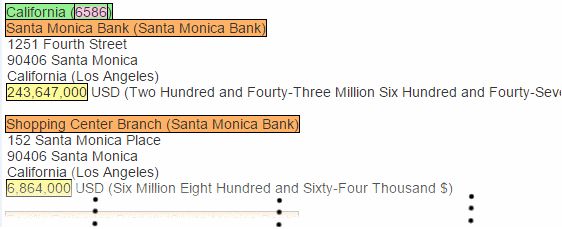
\includegraphics[width=0.8\columnwidth]{figures/bankinfo2}
    \caption{\BankListing: Highlighting sample.}
    \label{fig:interactive:evaluation:banksample}
\end{figure}

\begin{figure}[t]
    \centering
    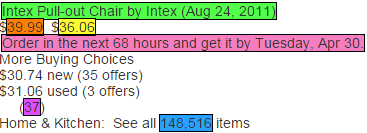
\includegraphics[width=0.6\columnwidth]{figures/amazon}
    \caption{Amazon research: Highlighting sample.}
    \label{fig:interactive:evaluation:amazonsample}
\end{figure}

\begin{figure}[t]
    \centering
    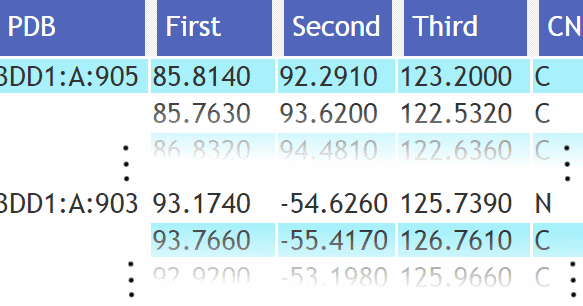
\includegraphics[width=0.6\columnwidth]{figures/hinthydrogens}
    \caption{Bioinformatic log: Result sample.}
    \label{fig:interactive:evaluation:biosample}
\end{figure}

\begin{figure}[t]
    \centering
    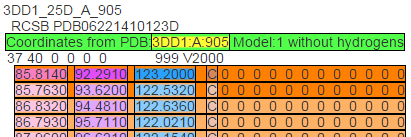
\includegraphics[width=0.7\columnwidth]{figures/hydrogenhybrid}
    \caption{Highlighting in the \InputTextView that produces the data in \Cref{fig:interactive:evaluation:biosample}.}
    \label{fig:interactive:evaluation:highlighting}
\end{figure}

After a brief tutorial, we ask users to perform extraction on the three files.
In order to measure the trust they give to the extraction, we do not tell them if their extraction is correct or not.
For each extraction task, we provide a result sample (such as \Cref{fig:interactive:evaluation:biosample}).
Users then manipulate \FlashProg to generate the entire output table corresponding to that task.

To answer \RQOneShort, we select a number of representative values across all fields
for each task, and we automatically measure how many of them were incorrectly highlighted.
These values were selected by running \FlashProg sessions in advance
ourselves and observing insightful checkpoints that require attention.
In total, we selected 6 values for task \#1, 13 for task \#2 and 12 for task \#3.
We do not notify users about their errors.
This metric has more meaning than if we recorded all errors.
As an illustration, a raw error measurement in the third task for a user forgetting about the third main record would
yield more than 140 errors.
Our approach returns 2 errors, one for the missing record, and one for another ambiguity that needed to be checked but
could not.
This makes error measurement comparable across tasks.

To measure the impact of \ProgramNavigation and \ConversationalClarification interaction models
independently, we set up three interface environments:

\begin{description}
    \item[\BIdef (\BI).] This environment enables only the PBE interaction model.
        It includes the following UI features: the labeling interface for mouse-triggered highlighting, the
        label menu to rename labels, to switch between them and the \OutputTab.
    \item[\BIPWdef (\BIPW).] Besides PBE, this interface enables the
        \ProgramNavigation interaction model, which includes the \ProgramNavigationTab and its features.
    \item[\BIDTdef (\BIDT).] Besides PBE, this environment enables the
        \ConversationalClarification interaction model, which includes the \ConversationalClarificationTab.
\end{description}

To compensate the learning curve effects when comparing the usefulness of various interaction models, we set up the
environments in three configurations A, B, and~C, shown in \Cref{tbl:playground:configurations}.
Each configuration has the same order of files/tasks, but we chose three environment permutations.
As we could not force people to finish the study, the number of users per environment is not perfectly balanced.

\begin{table}
    \centering
    \begin{tabular}{llllr} \toprule
        & \multicolumn{3}{c}{\textbf{Tasks}} & \\ \cmidrule(r){2-4}
        \multicolumn{1}{l}{\textbf{Configuration}} & \textbf{1. Bank} & \textbf{2. Amazon} & \textbf{3. Bio log} & \textbf{\# of users} \\ \midrule
        \multicolumn{1}{l}{\textbf{A}} & \BIPW & \BIDT & \multicolumn{1}{l}{\BI} & 8 \\
        \multicolumn{1}{l}{\textbf{B}} & \BI & \BIPW & \multicolumn{1}{l}{\BIDT} & 12 \\
        \multicolumn{1}{l}{\textbf{C}} & \BIDT & \BI & \multicolumn{1}{l}{\BIPW} & 9\\ \bottomrule
    \end{tabular}
    \caption{Configurations of the user study of user interaction models in \FlashProg.}
    \label{tbl:playground:configurations}
\end{table}

To answer \RQTwoShort{} and \RQThreeShort{}, we asked the participants about the
perceived usefulness of our novel interaction models, and the confidence
about the extraction of each file, using a Likert scale from 1 to 7, 1 being the
least useful/confident:

\begin{enumerate}[nosep]
    \item How confident were you in the final extraction result?
    \item After training, would you trust \FlashProg to work correctly on another similar file if you do not provide any
        examples?
    \item How easy was it for you to complete this task?
\end{enumerate}

\paragraph{Results}
We analyzed the data both from the logs collected by the UI instrumentation, and from the initial and final surveys.
% If a feature was activated, we counted the user for statistics even if he reported not using it.

\begin{figure}[t]
    \centering
    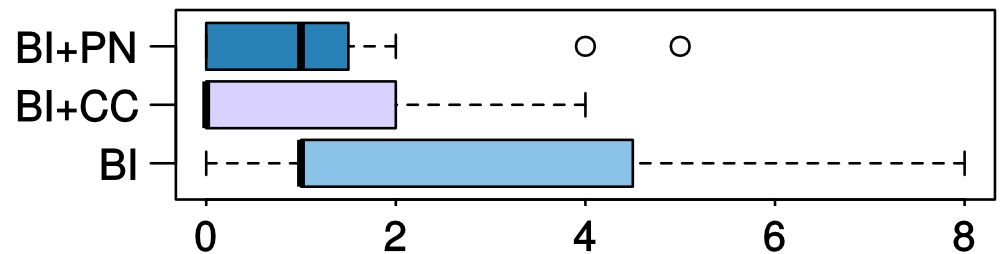
\includegraphics[width=0.6\columnwidth]{figures/error-plot1}
    \caption{Distribution of error counts across the three environments in the user study of data wrangling in
        \FlashProg.
        Both \ConversationalClarification{} (\ConversationalClarificationInitials) and
        \ProgramNavigation{} (\ProgramNavigationInitials) significantly decrease the number of errors.}
    \label{fig:interactive:study:errorcounts}
\end{figure}

\subsubsection*{\RQOneShort: \RQOne}
\textbf{Yes. We have found significant
reduction of number of errors with each of these new interaction models} (see \Cref{fig:interactive:study:errorcounts}).
Our new interaction models reduce the error rate in data extraction without any
negative effect on the users' extraction speed. To obtain this result, we applied the
Wilcoxon rank-sum test on the instrumentation data.
More precisely, users in \BIDT ($W=78.5$, $p=0.01$) and \BIPW ($W= 99.5$, $p=0.06$)
performed better than \BI, with no significant
difference between the two of them ($W=94$, \textit{n.s.}).
There was also no statistically significant difference between the completion time in \BI and
completion time in \BIDT ($W=178.5$, \textit{n.s.}) or \BIPW{} ($W=173$, \textit{n.s.}).

\subsubsection*{\RQTwoShort: \RQTwo}
\textbf{\ConversationalClarification is perceived more useful than \ProgramNavigation} (see
\Cref{fig:interactive:study:disambiguationuseful,fig:interactive:study:programnavigationuseful}).
Comparing the user-reported usefulness between the \ConversationalClarification and the \ProgramNavigation, on a
scale from 1 (not useful at all) to 7 (extremely useful), the
\ConversationalClarification has a mean score of \usefulnessDisambiguation{} ($\sigma =$
\usefulnessDisambiguationStdDev{})
whereas the \ProgramNavigation has \usefulnessProgramViewer{} ($\sigma =$ \usefulnessProgramViewerStdDev{})
Only \ifequal{\numUserPreferringProgramViewer}{1}{one user}{\numUserPreferringProgramViewer{} users} out of
\numPeopleSurvey{}
\ifequal{\numUserPreferringProgramViewer}{1}{scores}{score} \ProgramNavigation more useful than
\ConversationalClarification,
whereas \ConversationalClarification is scored more useful by
\numUserPreferringDisambiguation~\ifequal{\numUserPreferringDisambiguation}{1}{user}{users}.

\begin{figure}[t!]
    \centering
    \begin{subfigure}{\columnwidth}
        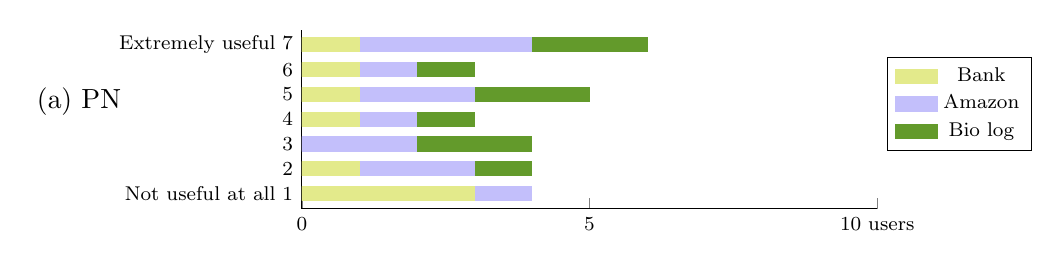
\begin{tikzpicture}[thick,scale=0.9]
            \begin{axis}[
                xbar stacked,
                legend style={
                    legend columns=1,
                    at={(0.85\columnwidth,0.05\columnwidth)},
                    anchor=south east
                },
                ytick=data,
                axis y line*=none,
                axis x line*=bottom,
                tick label style={font=\footnotesize},
                legend style={font=\footnotesize},
                label style={font=\footnotesize},
                xtick={0,5,10},
                xticklabels={0,5,10 users},
                width=.8\columnwidth,
                bar width=2mm,
                yticklabels={Extremely useful 7, 6, 5, 4, 3, 2, Not useful at all 1},
                xmin=0,
                xmax=\maxusersgraphs,
                area legend,
                y=3.5mm,
                ]
                \addplot[NumTaskOne,fill=NumTaskOne] coordinates
                    {\usefulnessProgramViewerTaskOne};
                \addplot[NumTaskTwo,fill=NumTaskTwo] coordinates
                    {\usefulnessProgramViewerTaskTwo};
                \addplot[NumTaskThree,fill=NumTaskThree] coordinates
                    {\usefulnessProgramViewerTaskThree};
                \legend{Bank, Amazon, Bio log};
            \coordinate (C) at (-31mm,11mm);
        \end{axis}
        \node at (C) {(a) PN};
    \end{tikzpicture}
    \phantomcaption
    \label{fig:interactive:study:disambiguationuseful}
\end{subfigure}
\begin{subfigure}{\columnwidth}
    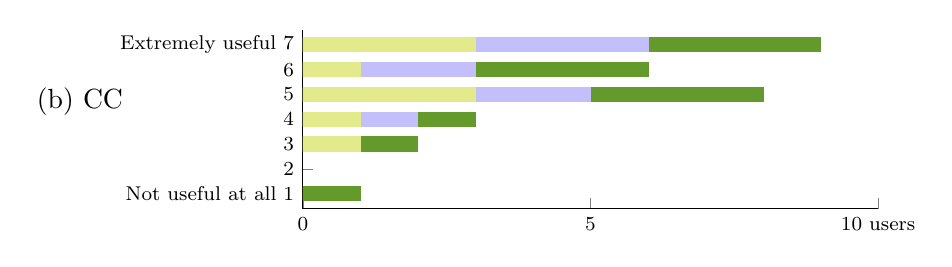
\begin{tikzpicture}[thick,scale=0.9]
        \begin{axis}[
            xbar stacked,
            legend style={
                legend columns=3,
                at={(xticklabel cs:0.5)},
                anchor=north,
                draw=none
            },
            ytick=data,
            axis y line*=none,
            axis x line*=bottom,
            tick label style={font=\footnotesize},
            legend style={font=\footnotesize},
            label style={font=\footnotesize},
            xtick={0,5,10},
            xticklabels={0,5,10 users},
            width=.8\columnwidth,
            bar width=2mm,
            yticklabels={Extremely useful 7, 6, 5, 4, 3, 2, Not useful at all 1},
            xmin=0,
            xmax=\maxusersgraphs,
            area legend,
            y=3.5mm,
            ]
            \addplot[NumTaskOne,fill=NumTaskOne] coordinates
                {\usefulnessDisambiguationTaskOne};
            \addplot[NumTaskTwo,fill=NumTaskTwo] coordinates
                {\usefulnessDisambiguationTaskTwo};
            \addplot[NumTaskThree,fill=NumTaskThree] coordinates
                {\usefulnessDisambiguationTaskThree};
            % \legend{Task 1, Task 2, Task 3}
            \coordinate (A) at (-31mm,11mm);
        \end{axis}
        \node at (A) {(b) CC};
    \end{tikzpicture}
    \phantomcaption
    \label{fig:interactive:study:programnavigationuseful}
\end{subfigure}
\begin{subfigure}{\columnwidth}
    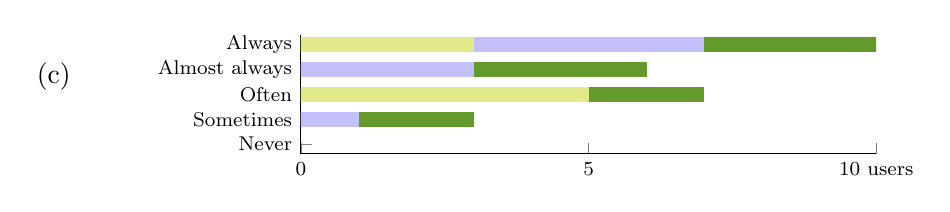
\begin{tikzpicture}[thick,scale=0.9]
        \begin{axis}[
            xbar stacked,
            legend style={
                legend columns=3,
                at={(xticklabel cs:0.5)},
                anchor=north,
                draw=none,
                draw=none
            },
            ytick=data,
            axis y line*=none,
            axis x line*=bottom,
            tick label style={font=\footnotesize},
            legend style={font=\footnotesize},
            label style={font=\footnotesize},
            xtick={0,5,10},
            xticklabels={0,5,10 users},
            width=.8\columnwidth,
            bar width=2mm,
            yticklabels={\phantom{Extremely} Always, Almost always, Often, Sometimes, Never},
            xmin=0,
            xmax=\maxusersgraphs,
            area legend,
            y=3.5mm,
            ]
            \addplot[NumTaskOne,fill=NumTaskOne] coordinates
                {\disambiguationCorrectnessTaskOne};
            \addplot[NumTaskTwo,fill=NumTaskTwo] coordinates
                {\disambiguationCorrectnessTaskTwo};
            \addplot[NumTaskThree,fill=NumTaskThree] coordinates
                {\disambiguationCorrectnessTaskThree};
            \coordinate (E) at (-34mm,8mm);
        \end{axis}
        \node at (E) {(c)};
    \end{tikzpicture}
    \phantomcaption
    \label{fig:interactive:study:disambiguationcorrect}
\end{subfigure}
\caption{User-reported: \textbf{(a)} usefulness of \ProgramNavigation, \textbf{(b)} usefulness of
    \ConversationalClarification, \textbf{(c)} correctness of one of the choices of \ConversationalClarification.}
\end{figure}

\subsubsection*{\RQThreeShort: \RQThree}
\textbf{Yes for \ConversationalClarification.}
The tasks finished with \ConversationalClarification
obtained a higher confidence score compared to those without ($W=181.5$, $p = 0.07$).
No significant difference was found for \ProgramNavigation ($W=152.5$, \textit{n.s.}).
Regarding the trust our users would have if they ran the learned program on
other data, we did not find any significant differences for
\ConversationalClarification ($W=146$, \textit{n.s.}) and \ProgramNavigation ($W=161$, \textit{n.s.}) over only \BI.

Regarding the question ``How often would you use \FlashProg, compared to
other extraction tools?'', on a Likert scale from 1 (never) to 5 (always), \preferredToHaveFlashProgFive{} users
answered 5, \preferredToHaveFlashProgFour{} answered 4, \preferredToHaveFlashProgThree{} answered 3, and the remaining
\preferredToHaveFlashProgTwoOrLess{} answered 2 or less.
Furthermore, \ifequal{\recommendFlashProgPercentage}{100}{all}{\recommendFlashProgPercentage\% of our users} would
recommend \FlashProg to others.
When asked how excited would they be to have such a tool on a scale from 1 to 5, \excitementPercentToHaveFlashProgFive{}
users answered~5, and \excitementPercentToHaveFlashProgFour{} answered 4.

The users' trust is supported by data: Perceived correctness is negatively correlated
with number of errors (Spearman $\rho=-0.25$, $p=0.07$).
Although we asked them to make sure the extraction is correct
and never told them they did errors, users making more errors  (thus unseen)
reported to be less sure about the extraction.
However, there is no significant correlation between number of errors made and
the programming experience mapped between 0 and 4 ($\rho=-0.09$, \textit{n.s.}).

\subsection{Conclusion}
The two key takeaways of this user study is that
\textbf{(a)} any user interaction model (\ProgramNavigation or \ConversationalClarification) reduces the number of
errors in the completed tasks and improves the users' confidence in the results (as compared to example-only workflow);
\textbf{(b)} \ConversationalClarification is perceived as more useful thanks to its proactivity and clarity.
Based on these observations, PROSE now includes a more general version of \ConversationalClarification (called
\emph{feedback-based synthesis}) as a key capability for any DSL.
The next section presents its design and applications.

\section{Feedback-Based Synthesis}
\label{sec:interactive:feedback}

As we discussed above, an end user often does not have a clear understanding of the full spec, and may suffer
significant cognitive load with this task.
At every iteration, the current candidate program set $\vsa_i$ contains thousands of ambiguous programs, and humans
struggle with reasoning about possible ambiguities in intent specification.
In contrast, the synthesis system can analyze ambiguities in $\vsa_i$ and derive the most efficient way to resolve them
by proactively soliciting concrete knowledge from the user.
This observation introduces a new actor in the traditional learner-user interaction process, which we call \emph{the
hypothesizer}.

\Cref{fig:feedback:hypothesizer} shows our envisioned workflow.
Formally, any \emph{constraint type} used in PBE (e.g. example, prefix, output type) states a \emph{property} on a
subset of the DSL.
Given a program set $\vsa_i$, the hypothesizer deduces possible properties that best disambiguate among programs in
$\vsa_i$.
Any such property is convertible to a Boolean or multiple-choice question $q$, which the hypothesizer asks the user.
Any response $r$ for $q$ is convertible to a concrete constraint $\constraint$, which begins a new iteration of
synthesis.

Such \emph{feedback-based} interaction has several major benefits.
First, it reduces the cognitive load on the user: instead of analyzing the program's behavior, she only answers concrete
questions.
Second, it significantly reduces the number of synthesis iterations thanks to the hypothesizer's insight into the
program set $\vsa$ and its choice of disambiguating questions.
Finally, feedback and proactiveness increases the user's confidence and trust in the system.

\tikzstyle{flowchart} = [semithick, align=center, >=stealth', every path/.style={->, font=\small}]
\tikzstyle{actor} = [draw, rounded corners, inner sep=6pt, node distance=2cm, font=\sffamily, outer sep=3pt,
                     fill=blue!20]
\tikzstyle{data} = [inner sep=5pt]
\tikzstyle{empty} = [inner sep=0pt, outer sep=0pt]
\tikzstyle{pass} = [densely dashed, thin, >=spaced open triangle 45, color=gray]
\tikzstyle{edgelabel} = [sloped, anchor=center, above]

\begin{figure}[t]
    \centering
    \begin{tikzpicture}[flowchart]
        \node [actor] (learner) {Learner};
        \node [actor, right=3cm of learner] (user) {User};
        \path (learner) to coordinate[midway] (mid) (user);
        \node [actor, above=3.0cm of mid] (analyzer) {Hypothesizer};
        \node [data, left=of learner] (ranking) {Ranking function $h$};
        \draw (ranking) to (learner);
        \draw (learner) to ["VSA $\vsa$" {edgelabel, pos=0.33}, bend left=20]
            node[empty, pos=0.85] (lstart) {}
            (analyzer);
        \draw (user) to["spec $\spec$"]
            node[empty, pos=0.85] (rend) {}
            (learner);
        \node [data, above left=1.2cm and 1.0cm of learner] (dsl) {DSL $\dsl$};
        \draw (dsl) to
            node[empty, midway] (lend) {}
            (learner);
        \draw (analyzer.south east) to["question $q$" edgelabel, bend left=10] (user);
        \draw (user) to["response $r$" {edgelabel, below, pos=0.37}, bend left=10]
            node[empty, pos=0.88] (rstart) {}
            ($(analyzer.south east) - (0.4,0)$);
        \draw[pass] (rstart) to["refined spec $\spec'$"' edgelabel, bend right=20] (rend);
        \draw[pass] (lstart) to["refined DSL $\dsl'$"' edgelabel, bend right=30] (lend);
    \end{tikzpicture}
    % \uwsinglespace
    \caption{Learner-user communication in interactive PBE.
        At each iteration, the hypothesizer takes from the learner the VSA $\vsa$ of the programs consistent with the
        current spec $\spec$, and performs two automatic optimizations:
        (i) it converts the VSA into a refined DSL $\dsl'$ to be used at the next iteration instead of the original DSL
        $\dsl$, and
        (ii) it constructs the most effective clarifying question $q$ to ask the user about the ambiguous candidates in
        $\vsa$, and converts the user's response $r$ into the corresponding refined spec $\spec'$.}
    \label{fig:feedback:hypothesizer}
\end{figure}


\paragraph{Correctness-burden balance}
The crucial part of the hypothesizer's job is evaluation of disambiguation effectiveness of every potential question.
Our prototype implementation of \ConversationalClarification in \FlashProg always requested its clarification on the
first available discrepancy.
However, this is neither the fastest nor the most user-friendly experience:
\begin{itemize}
    \item On one hand, a system might ask for an additional example every time there exists an alternative candidate
        program that disagrees with the current most likely candidate on some row.
        In this case, the learning session is guaranteed to converge to the desired program if one exists, typically
        within 10-20 iterations.

        Despite the attractive guarantee, this approach is undesirable because a good ranking function often picks the
        intended program after 1-5 examples.
        In such a case, all subsequent iterations only eliminate implausible candidates without actually changing the
        result.
        The user spends a lot of cognitive effort answering superfluous questions.

    \item On another hand, the system might stop asking disambiguating questions too early.
        In this case, the learned program may be incorrect but the user will only notice it if she discovers a
        discrepancy manually.
\end{itemize}
In machine learning terminology, a superfluous disambiguating question is a \emph{false positive} (it is generated but
not strictly required to learn the correct program), and a missing disambiguating question is a \emph{false negative}
(it is required but not generated).
Our \FlashProg study~\cite{flashprog} included only the most conservative disambiguating algorithm, which always
converged to zero ambiguities.
As a result, it always generated false positive questions.

To minimize false positives, a disambiguating algorithm must intelligently pick the discrepancies presented to the user.
Well-chosen discrepancies will eliminate implausible candidate programs from consideration faster.
To minimize false negatives, the algorithm must intelligently estimate the likelihood of the currently chosen candidate
program.
A good estimation should ensure that any correct (or at least plausible) program is ranked higher than all incorrect
(implausible) programs.

\subsection{Problem Definition}
Let $\dsl$ be a DSL.
Let $\Psi$ be a set of top-level \emph{constraint types} supported by the synthesizer and witness functions for $\dsl$.
For each constraint type $\constraint \in \Psi$ we associate a \emph{descriptive question} $q$ such that a
response $r$ for this question directly constitutes an instance of~$\constraint$.
We denote such a constraint as $\Psi(r)$.
Questions $q$ can be Boolean (usually in ternary logic) or multiple-choice.
We denote the set of possible responses for $q$ as $R(q)$.

\begin{example}
    An \emph{example constraint} ``output $= v$'' corresponds to a multiple-choice question ``Is the desired output on
    an input $\state$ equal to $v_1, v_2, \dots, \text{ or } v_k$?''
    A response to this question constitutes an example constraint ``output $= v_i$'' for the chosen $i$.

    A \emph{datatype constraint} ``$\text{output}\colon \tau$'' corresponds to a Boolean question ``Is the desired
    program a computation of type $\tau$?
    Yes (always), no (never), or unknown (maybe).''

    Questions, like constraints, can be domain-specific.
    In FlashFill, a \emph{relevance constraint} states ``an input $v_i$ must/must not appear in the program.''
    It corresponds to a Boolean question ``Should the input $v_i$ be used?
    Yes (always), no (never), or unknown (maybe).''
\end{example}

\begin{figure}[t]
    \centering
    \uwsinglespace
    \begin{algorithmic}[1]
        \NoNumber \Procedure{Disambiguate}{Candidate programs $\vsa$, current spec $\spec$}
        \addtocounter{ALG@line}{-1} \WithNumber
        \State Analyze the ambiguities in $\vsa$ w.r.t.
$\spec$.
        \Statex Let $Q$ be a set of questions that may resolve ambiguity in $\vsa$
        \Statex \Comment{Compare the disambiguation scores of all questions}
        \State $q^{*} \gets \argmax\limits_{q \in Q} \mathsf{ds}(q, \vsa, \spec) $
        \If{$\mathsf{ds}(q^{*}, \vsa, \spec) < \text{threshold } T$}
        \State \textbf{break}
        \Else
        \State Present the question $q^{*}$ to the user
        \State Let $r$ be the user's response to $q$
        \State Let $\constraint$ be the response $r$ converted into a constraint
        \State \Return $\constraint$ to the learner and invoke a new round of synthesis
        \EndIf
        \EndProcedure
    \end{algorithmic}
    \vspace{\baselineskip}
    \caption{The hypothesizer's proactive disambiguation algorithm.}
    \label{fig:feedback:algorithm}
\end{figure}

\Cref{fig:feedback:algorithm} shows the disambiguation algorithm of the hypothesizer.
Given a VSA $\vsa$ of current candidate programs and the current iteration's spec $\spec$, the job of the hypothesizer
is to analyze~$\vsa$ and pick the best question to resolve ambiguities in~$\vsa$.
If~$\vsa$ has no ambiguities, or if the hypothesizer is not confident in the effectiveness of potential questions, it
considers the current candidate program $P^{*} = \mathsf{Top}_h \left(\vsa, 1\right)$ correct and does not ask any
questions.

\subsection{Disambiguation Score}

To evaluate a question's effectiveness, the hypothesizer is parameterized with a \emph{disambiguation score} function
$\mathsf{ds}(q, \vsa, \spec)$.
Higher disambiguation scores correspond to more effective questions $q$ -- that is, constraints generated by answering
$q$ eliminate more incorrect programs from $\vsa$.
Since the hypothesizer cannot predict the user's response, $\mathsf{ds}(q, \vsa, \spec)$ must represent \emph{potential
effectiveness} of $q$ for any possible outcome.

Disambiguation score functions may be domain-specific or general-purpose.
In our evaluation, we found different functions to perform well for different DSLs.
In this section, I present two efficient \emph{general-purpose} disambiguation score function.
One of them is independent of the current iteration's spec $\spec$ but takes into account the ranking scores of
alternative candidate programs in $\vsa$.
Another one is independent of any domain-specific details of the DSL (including its ranking function), but may be harder
to compute.

\paragraph{Ranking-based disambiguation}
The \emph{ranking-based disambiguation score} function prefers a question that promotes higher-ranked programs:
\[
    \mathsf{ds_R}(q , \vsa, \spec) \bydef \min_{r \in R(q)} \max_{P \in \vsa_r} h(P)
\]
where $\vsa_r$ is a set projection $\mathsf{Filter}\left(\vsa, \Psi(r)\right)$, and $h$ is a ranking function provided
with the DSL.
In other words, $\mathsf{ds_R}(q , \vsa, \spec)$ is higher if every response for the question $q$ leads to a
higher-ranked alternative program among the candidates that are consistent with it.

This disambiguation score can be efficiently evaluated for many constraint types.
For instance, calculating $\mathsf{ds_R}(q , \vsa, \spec)$ for \emph{example constraints} amounts to clustering $\vsa$
and comparing the top-ranked programs across all clusters.
Alternatively, we can quickly compute a good approximation to $\mathsf{ds_R}(q , \vsa, \spec)$ by randomly sampling $k$
programs from the VSA and considering only their outputs.

\paragraph{Entropy-based disambiguation}
The \emph{entropy-based disambiguation score} prefers a question that resolves more uncertainty in the VSA:
\[
    \mathsf{ds_E}(q , \vsa) = E \left\{ \vsa_r \,\middle|\, r \in R(q) \right\}
\]
where each $\vsa_r$ is a \emph{projection} of $\vsa$ onto the corresponding constraint for the response $r$:
\[
    \vsa_r = \mathsf{Filter}\left(\vsa,\, \Psi(r)\right)
\]
and $E(\vsa_1, \dots, \vsa_k)$ is the \emph{entropy of sizes} of its parameters:
\[
    E(\vsa_1, \dots, \vsa_k) = - \sum_{i=1}^k \frac{|\vsa_i|}{Z} \log \frac{|\vsa_i|}{Z}, \qquad
    Z = |\vsa_1| + \dots + |\vsa_k|
\]
In other words, $\mathsf{ds_E}(q , \vsa)$ is higher if possible responses for $q$ induce a high-entropy partitioning of
$\vsa$ (i.e., they split $\vsa$ into fairly even partitions).

\begin{example}
    If $q$ is a question for an \emph{example constraint}, its set of responses $R(q)$ includes all possible outputs
    $r_1, \dots, r_k$ of the programs currently in $\vsa$.
    The corresponding constraint $\Psi(r_j)$ for each response is the example constraint ``output $= r_j$''.
    Thus, the projections $\mathsf{Filter}\left(\vsa, \Psi(r_1)\right), \dots, \mathsf{Filter}\left(\vsa,
    \Psi(r_k)\right)$ are simply clusters in the partitioning $\clustering$ of $\vsa$ w.r.t. the current input $\state$.
    Each of the clusters contains only the programs that evaluate to the same output $r_j$.

    Hence, $\mathsf{ds_E}(q , \vsa)$ in this case is equal to the entropy of the clustering $\clustering$.
    Given a VSA $\vsa$, the hypothesizer simply computes its clustering on the current input $\state$, computes the
    entropy of this clustering, and uses it to decide the potential effectiveness of asking a multiple-choice
    disambiguation question.

    For example, consider a VSA of 10 programs that produce 2 different outputs.
    $R(q)$ then has two options, one for each possible output.
    If the cluster sizes corresponding to these outputs are $\{5; 5\}$, then the entropy of this clustering is high, and
    any response to $q$ will eliminate a significant fraction of the candidate programs.
    In contrast, if the cluster sizes are $\{9; 1\}$, then the entropy of this clustering is low, and a response may or
    may not be efficient in eliminating incorrect programs.
\end{example}

\begin{example}
    For a ternary Boolean question $q$ (e.g., a datatype question) the response set $R(q) = \left\{\text{``yes''},
        \text{``no''}, \text{``unknown''}\right\}$.
    The first two responses split $\vsa$ into two disjoint partitions.
    The third response does not provide any new information, so its corresponding projection is the entire $\vsa$, which
    contributes 0 to the entropy summation.
    Therefore, $\mathsf{ds_E}(q , \vsa)$ is equal to the entropy of the two-way split of $\vsa$ into programs satisfying
    $q$ and all others.
\end{example}

As compared to ranking-based disambiguation score, the entropy-based score is independent of a ranking function and
therefore DSL-agnostic.
However, it also has its drawbacks, such as reliance on the clustering operation $\clustering$, which may be expensive
for large VSAs.
% We evaluate the effectiveness of both disambiguation scores in \Cref{sec:evaluation}.

\subsection{Evaluation}

We use the PROSE-based implementation of FlashFill to evaluate feedback-based synthesis on a set of 457 text
transformation tasks.
It uses \emph{example} constraint questions.
In order to efficiently generate these questions, we sample $2000$ programs from the VSA and cluster on those, assigning
the disambiguation score $\mathsf{ds_R}$ as described above.
We chose $2000$ to achieve a good balance between performance and having a high probability of including
at least one program from every large cluster.

In the \emph{baseline setting}, the user provides the earliest incorrect row as the next example at each iteration.
In the \emph{feedback-driven setting}, the system instead proactively asks the user disambiguating questions on selected
input rows until the disambiguation score falls below the threshold $T$.
We set $T = 0.47$ as the mean of the score distribution over our tasks.

We evaluate FlashFill's feedback on two dimensions: \emph{cognitive burden} and \emph{correctness}.
Cognitive burden is defined as the number of rows the user has to \emph{read and verify} in the process.
In the baseline setting, it is the number of examples $+$ the number of correct rows before the first discrepancy that
are verified at each iteration.
In the feedback-driven setting, it is the number of questions answered.

Correctness is a combination of \emph{false positives} and \emph{false negatives}.
False positive questions occur when FlashFill keeps asking questions after the program is already correct.
False negative questions occur when FlashFill stops before it finds a correct program.

In correctness evaluation, only 2/457 tasks completed incorrectly (i.e., with false negatives).
The majority of tasks (342/457) finish with the same number of examples, and the number of false positives in the rest
never exceeds 4 (specifically, 90 tasks with 1 false positive, 22 with 2, and 1 task with 4 false positives).

\begin{table}[t]
    \centering
    \begin{tabular}{llllll}
        \toprule
        & \multicolumn{5}{c}{\textbf{Feedback-driven}} \\
        \cmidrule{2-6}
        \textbf{Baseline} & \textbf{1} & \textbf{2} & \textbf{3} & \textbf{4} & \textbf{5} \\
        \midrule
        \textbf{1} & 241 & 50 & 16 &   & 1 \\
        \textbf{2} & 75 & 30 & 4 &   &   \\
        \textbf{3} & 20 & 7 & 2 &   &   \\
        \textbf{4} &   & 5 & 3 &   &   \\
        \textbf{5} &   & 1 &   &   &   \\
        \textbf{6} & 1 & 1 &   &   &   \\
        \bottomrule
    \end{tabular}
    \uwsinglespace
    \caption{Number of rows inspected in the baseline and the feedback-driven settings for the evaluation of
        a feedback-driven FlashFill interaction with a ranking-based disambiguation score.
        The data is presented as a histogram: for example, there were \textbf{20/457} scenarios such that the baseline
        setting required \textbf{3} iterations to complete the task, and the feedback-based setting required \textbf{1}
        iteration.
        Empty cells represent the value of $0$.}
    \label{tbl:feedback:ff:iterations}
\end{table}

\Cref{tbl:feedback:ff:iterations} compares the cognitive burden of both settings.
It shows the histogram distribution of our tasks for each pair of verified row counts in baseline and feedback-driven
settings.
The baseline setting often requires the user to inspect more rows (that is, the numbers \emph{below} the diagonal in
\Cref{tbl:feedback:ff:iterations} are larger than the numbers above it).
\todoinline{Evaluation of the entropy-based disambiguation.}

\section{Incremental Synthesis}
\label{sec:interactive:incremental}

